\section{Fallbeispiel 2 -- Aktuelle Meldungen}
    Dieses Fallbeispiel klassifiziert Übersichtsseiten mit aktuellen
    Meldungen der Fakultät \gls{ksw} der {\fernUni}.
    Wie im vorherigen Beispiel wird dazu zunächst eine dieser Seiten analysiert,
    ein konzeptionelles Modell erstellt
    und anschließend das {\classificationModel} erläutert.

    Die Klassifizierung wurde nicht auf allen Sites wiederholt,
    da dadurch keine neuen Erkenntnisse zu erwarten waren.
    Anders als im ersten Fallbeispiel besitzt eine einzelne Site aber
    mehrere Nachrichtenseiten,
    weshalb alle Seiten\footnote{Zum Zeitpunk des Versuchs besaß die Site fünf Nachrichtenseiten}
    des Portals \gls{babw} klassifiziert und die Ergebnisse in einer gemeinsamen Datenbank gespeichert
    wurden.
    
    Wie zuvor werden zu diesem Versuch sowohl einige Kennzahlen
    als auch Unregelmäßigkeiten der Klassifikationen präsentiert.

    \subsection{Konzeptionelles Modell der Webseite}
    \label{section:findingsTeachersConceptualModel}
    Das konzeptionelle Modell wird in diesem Beispiel anhand
    der Übersichtsseite des Studienportals \gls{babw} beschrieben.
    Abbildung \ref{image:findingTeachersModelOverview} zeigt einen
    Ausschnitt dieser Seite, auf dem die wichtigsten Bereiche zu sehen sind.
    Eine Darstellung des Modells ist in Abbildung
    \ref{image:findingTeachersModelUml} zu sehen.

    \begin{figure}[htb]
        \centering
        
\includegraphics[width=\textwidth]{../resources/findings/case-study-1/model/overview.png}
        \caption{Die Webseite über Mitarbeiter des Portals \acrshort{babw}}
        \label{image:findingTeachersModelOverview}
    \end{figure}

    Die Webseite lässt sich in verschiedene Bereiche aufteilen.
    Zunächst einen Kopfbereich, der auf der linken Seite das Logo
    der {\fernUni} enthält.
    Dieses Bild ist gleichzeitig ein Link zur Hauptseite der Universität. 
    Auf der rechten Seite enthält der Kopfbereich einige Links zu den verschiedenen
    Bereichen der Site.
    Direkt unter dem Kopfbereich befindet sich der Name des Studienportals,
    welcher gleichzeitig ein Link auf die Einstiegsseite des Portals ist.
    Darunter befindet sich auf der linken Seite ein weiterer Navigationsbereich,
    der Verweise auf die Unterseiten des aktuellen Bereichs enthält.
    Rechts daneben findet sich zunächst der Titel der Seite,
    gefolgt von einem kurzen einleitenden Absatz.
    Alle bisher genannten Elemente der Seite finden sich in sehr ähnlicher Form
    auch auf anderen Seiten wieder.
    Die dem einleitenden Absatz folgende Liste aller Lehrenden und Betreuenden unterscheidet die Seite hingegen von anderen.
    Für jeden Mitarbeiter sind eine Reihe an Informationen dargestellt.
    Neben einem Bild ist das der Name des Lehrgebiets, in dem er tätig ist.
    Dieser Name ist außerdem ein Link auf eine Seite über dieses Gebiet.
    Es folgen der Name des Mitarbeiters
    und einige Kontaktinformationen.
    Dies können eine E-Mail-Adresse, eine Telefonnummer
    und bei einigen wenigen Kontakten auch eine Faxnummer und ein Raum sein.

    \begin{figure}[htb]
        \centering
        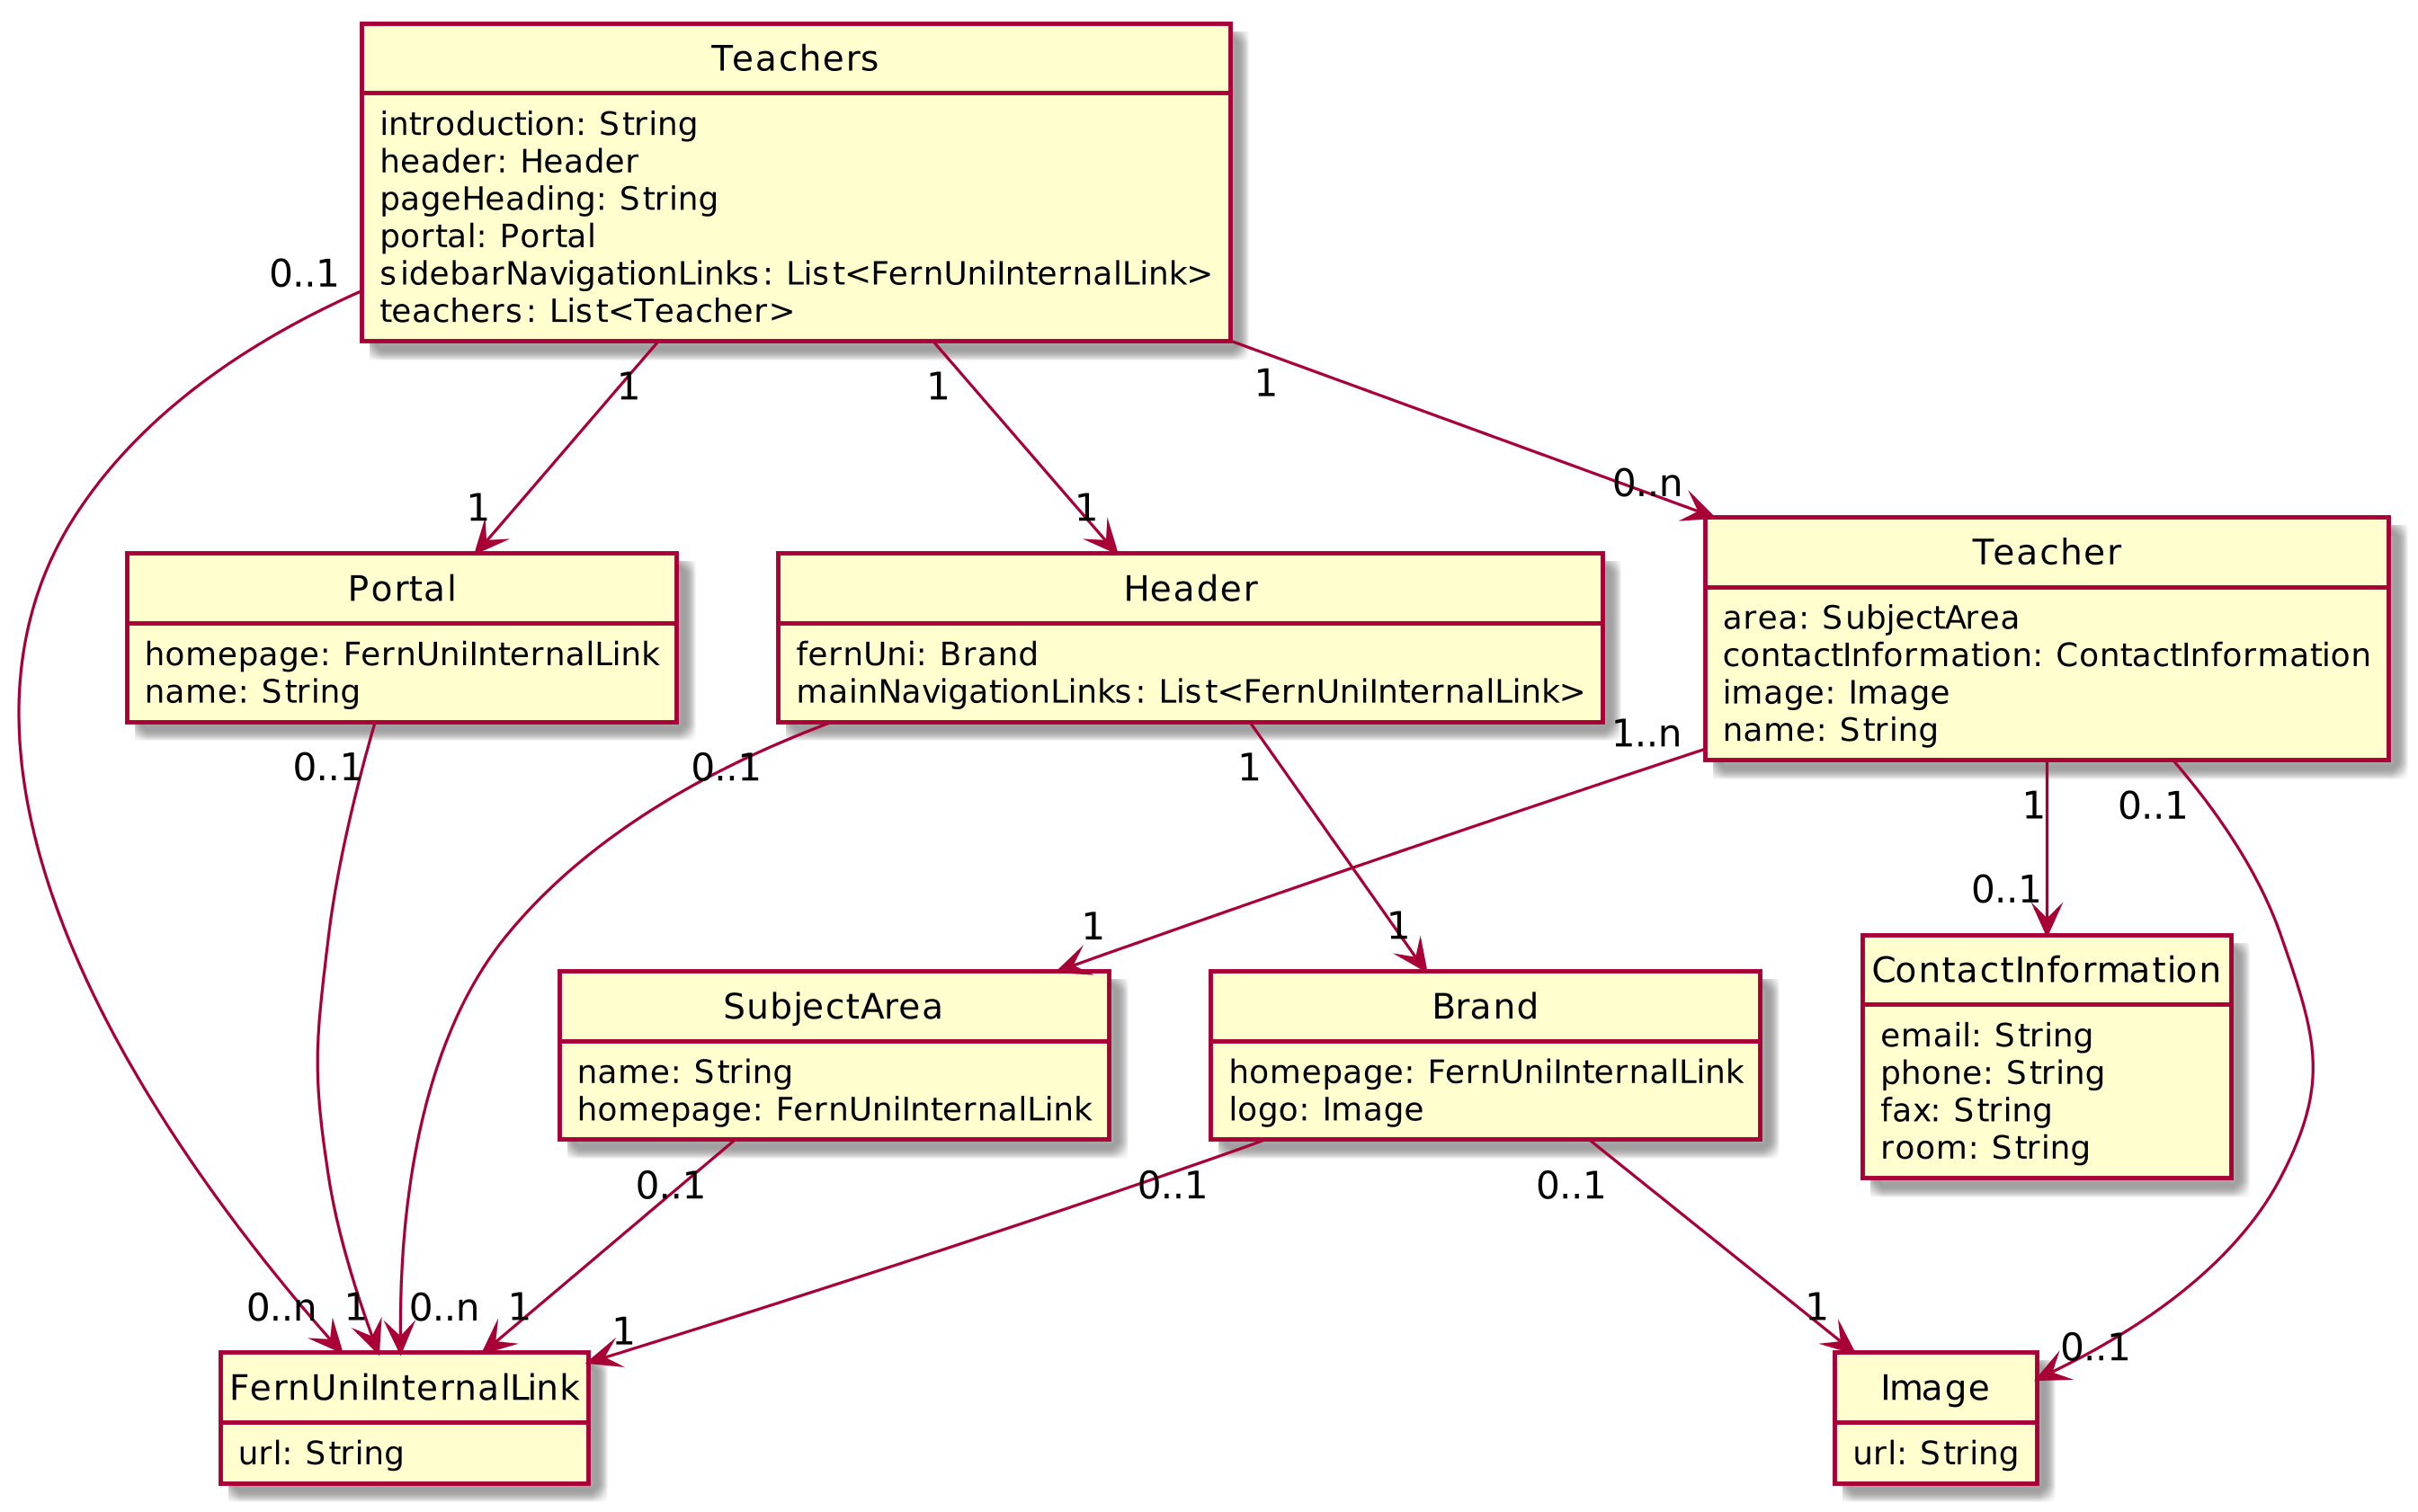
\includegraphics[scale=\imageScalingFactor]{../resources/findings/case-study-1/model/model.png}
        \caption{Das konzeptionelle Modell einer Webseite über Mitarbeiter}
        \label{image:findingTeachersModelUml}
    \end{figure}
    \subsection{Das {\classificationModel}}
    \label{section:findingsNewsClasses}
    Bei der Analyse der Nachrichtenseite wurde deutlich,
    dass einige Teile konzeptionell identisch mit denen aus dem ersten Beispiel sind.
    Die allgemeinen Klassendefinitionen aus Listing \ref{listing:findingsTeachersCommon}
    werden deshalb hier wiederverwendet.
    Die speziellen Definitionen für Nachrichtenseiten sind in
    Listing \ref{listing:findingsNewsSpecial}
    aufgeführt\footnote{Der Selektor in den Zeilen \ref{line:newsWctdInvalidSelectorStart}
    bis \ref{line:newsWctdInvalidSelectorEnd} wurde aus Gründen der Lesbarkeit umgebrochen,
    was syntaktisch nicht erlaubt ist.}.

    \lstinputlisting[
        label=listing:findingsNewsSpecial,
        caption=Das {\classificationModel} der Webseite \"uber aktuelle Meldungen,
        language=wccdl,
        inputencoding=utf8/latin1,
        style=wccdl,
        escapechar=|
    ]{../resources/findings/case-study-2/classification-model/NewsOverview.wctd}

    Die Seitenklasse \texttt{NewsOverview} enthält Features für die
    allgemeinen Bereiche der Seite sowie für die Referenzen auf die vorherige und die nächste
    Nachrichtenseite. Diese {\referenceFeature}s werden alle als \texttt{FernUniInternalLink} klassifiziert.
    Nicht zuletzt besitzt \texttt{NewsOverview} ein {\collectionFeature} für die Meldungen.
    Eine Nachricht wird durch die Klasse \texttt{News} repräsentiert,
    ihr Datum durch \texttt{NewsDate}, ihre Überschrift durch \texttt{NewsHeading}
    und ihre Absätze durch \texttt{NewsSection}.
    Die Überschrift enthält auch einen Link,
    der ebenfalls als \texttt{FernUniInternalLink} klassifiziert wird.
    Das Feature \texttt{sections} wurde auskommentiert.
    Der Grund ist, dass für die Absätze einer Nachricht kein Selektor ermittelt werden konnte,
    mit dem eine sinnvolle Klassifizierung möglich ist.
    Um dies zu erklären, ist eine Betrachtung der \gls{html}-Struktur der Nachrichtenliste notwendig.
    Diese Struktur ist in Listing \ref{listing:findingsNewsEvilHtmll}
    zu sehen, wobei konkrete textuelle Inhalte entfernt wurden,
    da sie für das Verständnis der Problematik irrelevant sind.

    \lstinputlisting[
        label=listing:findingsNewsEvilHtmll,
        caption=Die HTML-Repräsentation der Nachrichtenliste der Seiten über aktuelle Meldungen,
        style=html
    ]{../resources/findings/case-study-2/news.html}

    Aus diesem Fragment geht hervor,
    dass Nachrichten nicht in einzelne \gls{html}-Elemente gekapselt sind.
    Stattdessen befinden sich alle Elemente aller Nachrichten auf derselben Hierarchieebene.
    Nachrichten werden nur durch ein \texttt{hr}-Element voneinander getrennt,
    was sich das {\classificationModel} zunutze machen kann.
    Aufgrund der fehlenden Kapselung ist es aber mit den zur Verfügung
    stehenden CSS- und XPath-Selektoren nicht möglich festzustellen,
    welche Elemente als \texttt{NewsSection} zu klassifizieren sind.
    Der {\cssSelector} \texttt{p} würde bspw. alle Absätze aller Nachrichten selektieren.
    Erschwerend kommt hinzu, dass Absätze nicht nur \texttt{p},
    sondern auch andere Elemente sein können und dass jede Nachricht eine andere Anzahl an Absätzen besitzt.
    Informell ausgedrückt wäre ein Selektor notwendig,
    der ausgehend vom aktuellen Kontextelement (das \texttt{hr}-Element) alle Elemente
    ab dem ersten \texttt{h4}-Element bis zum nächsten \texttt{hr} selektiert.
    Das ist mit CSS nicht möglich, da es keine Selektoren für Geschwister des Kontextelementes gibt.
    XPath besitzt diese zwar, allerdings konnte auch mit diesen kein
    Ausdruck umgesetzt werden, der nur die Absätze der aktuellen Nachricht herausfiltert.
    Die einzige Lösung -- ohne das HTML anzupassen -- ist für jede Nachricht eine spezielle Klasse zu entwickeln.
    Durch eine solche 1:1-Beziehung kann jede Klasse individuelle und gleichzeitig
    eindeutige Selektoren für die Absätze enthalten.

    \subsection{Kennzahlen}
    Auch in diesem Fallbeispiel wurde eine Reihe an Kennzahlen ermittelt,
    die in diesem Kapitel präsentiert werden.

    \paragraph{Struktur eines Graphs}
    Zum Verständnis der Zahlen trägt Abbildung \ref{image:findingNewsFiguresDbModel} bei,
    welches den Aufbau des Graphs visualisiert.
    Wegen der beschriebenen Überschneidung mit dem ersten Fallbeispiel,
    sind die entsprechenden Knoten hier nicht nochmals dargestellt.
    Wie im vorherigen Beispiel wird außerdem auf die Darstellung von
    Referenzen verzichtet.

    \begin{figure}[htb]
        \centering
        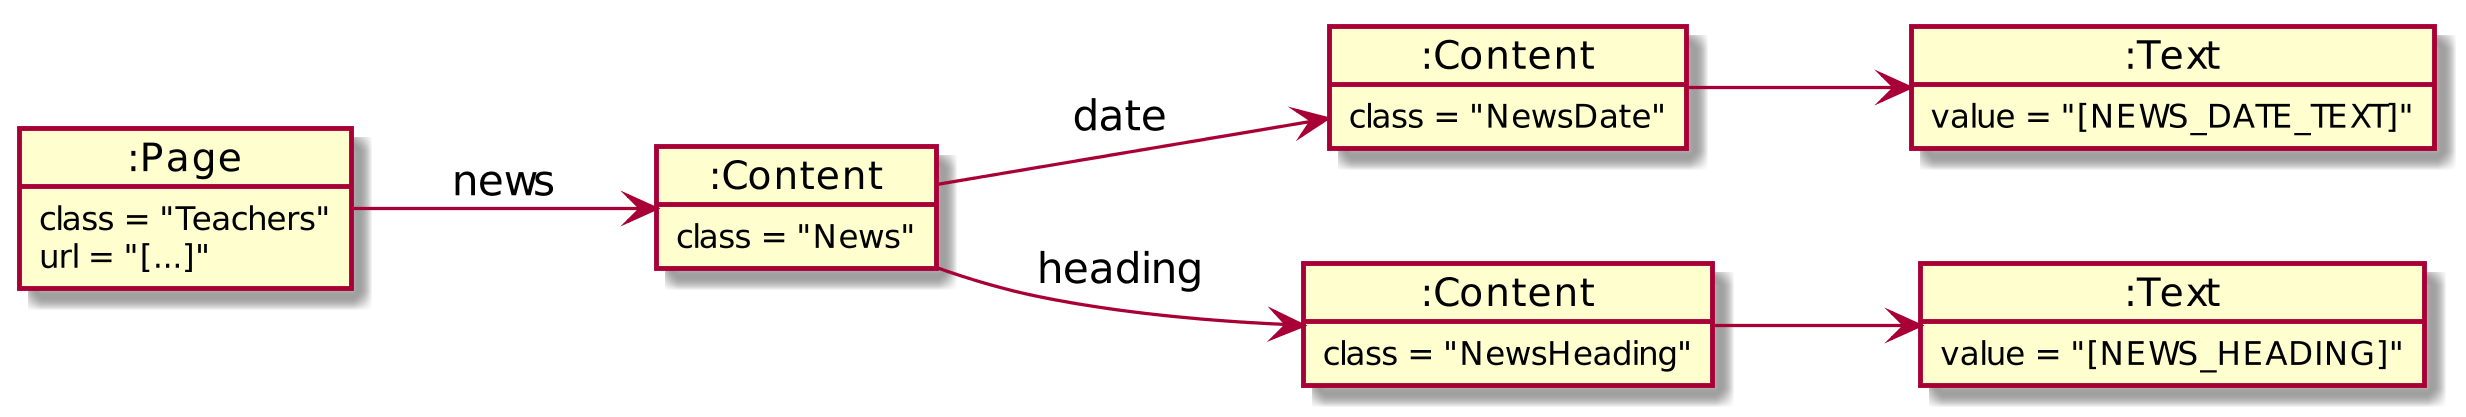
\includegraphics[scale=\imageScalingFactor]{../resources/findings/case-study-2/dbmodel.png}
        \caption{Struktur des Graphs einer Seite über aktuelle Meldungen}
        \label{image:findingNewsFiguresDbModel}
    \end{figure}

    \paragraph{Präsentation der Kennzahlen}
    Die folgenden Tabellen präsentieren die gesammelten Kennzahlen.
    Die Bedeutung einzelner Kennzahlen wurde bereits beim ersten Beispiel erläutert,
    die entsprechend auch hier gelten.
    Die Gruppierung der Knoten nach ihren Labels ist in Tabelle
    \ref{table:findingsNewsFiguresNodesByLabel} zu sehen.
    Die Häufigkeit der Inhaltsklassen stellt Tabelle
    \ref{table:findingsNewsFiguresContentNodesByClass} dar.
    Tabelle \ref{table:findingNewsFiguresEdgesByLabel} gruppiert die Kanten der Datenbank
    nach ihren Labels und Tabelle
    \ref{table:findingsNewsFiguresEdgesByStartEndNodeLabel}
    stellt heraus, welche Knotenarten diese Kanten verbinden.
    Zuletzt betrachtet Tabelle \ref{table:findingsNewsFiguresSharedNodes}
    die Frage, welche Knoten mehrfach referenziert wurden.

    \begin{table}[htb]
        \begin{subtable}[c]{0.3\textwidth}
            \centering
            \begin{tabular}{|l|c|}
                \hline
                \textbf{Label}  & \multicolumn{1}{l|}{\textbf{Anzahl}} \\ \hline
                Content         & 124                                  \\ \hline
                Page + Resource & 5                                    \\ \hline
                Resource        & 53                                   \\ \hline
                Site            & 1                                    \\ \hline
                Text            & 77                                   \\ \hline
                \hline
                \textbf{Summe}  & 260                                  \\ \hline
            \end{tabular}
            \subcaption{Knoten gruppiert nach Labels für Seiten über aktuelle Meldungen}
            \label{table:findingsNewsFiguresNodesByLabel}
        \end{subtable}
        \begin{subtable}[c]{0.3\textwidth}
            \centering
            \begin{tabular}{|l|c|}
                \hline
                \textbf{Klasse} & \multicolumn{1}{l|}{\textbf{Anzahl}} \\ \hline
                Brand           & 1                                    \\ \hline
                Header          & 1                                    \\ \hline
                News            & 41                                   \\ \hline
                NewsDate        & 38                                   \\ \hline
                NewsHeading     & 41                                   \\ \hline
                PageHeading     & 1                                    \\ \hline
                Portal          & 1                                    \\ \hline
                \hline
                \textbf{Summe}  & 260                                  \\ \hline
            \end{tabular}
            \subcaption{\texttt{Content}-Knoten gruppiert nach ihrer Klasse für Seiten über aktuelle Meldungen}
            \label{table:findingsNewsFiguresContentNodesByClass}
        \end{subtable}
        \begin{subtable}[c]{0.3\textwidth}
            \centering
            \begin{tabular}{|l|c|}
                \hline
                \textbf{Label} & \multicolumn{1}{l|}{\textbf{Anzahl}} \\ \hline
                Reads          & 80                                   \\ \hline
                References     & 87                                   \\ \hline
                Owns           & 145                                  \\ \hline
                \hline
                \textbf{Summe} & 312                                  \\ \hline
                \end{tabular}
            \subcaption{Kanten gruppiert nach Labels für Seiten über aktuelle Meldungen}
            \label{table:findingNewsFiguresEdgesByLabel}
        \end{subtable}

        \begin{subtable}[c]{0.5\textwidth}
            \centering
            \begin{tabular}{|l|c|}
                \hline
                \textbf{Start $\rightarrow$ Ziel} & \multicolumn{1}{l|}{\textbf{Anzahl}} \\ \hline
                (:Content) $\rightarrow$ (:Content)     & 83                                   \\ \hline
                (:Content) $\rightarrow$ (:Resource)    & 49                                   \\ \hline
                (:Page) $\rightarrow$ (:Content)        & 57                                   \\ \hline
                (:Page) $\rightarrow$ (:Page)           & 13                                   \\ \hline
                (:Page) $\rightarrow$ (:Resource)       & 25                                   \\ \hline
                (:Site) $\rightarrow$ (:Page)           & 5                                    \\ \hline
                \textbf{Summe}                    & 232                                  \\ \hline
            \end{tabular}
            \subcaption{Kanten gruppiert nach Labels der Start- und Zielknoten für Seiten über aktuelle Meldungen}
            \label{table:findingsNewsFiguresEdgesByStartEndNodeLabel}
        \end{subtable}
        \begin{subtable}[c]{0.5\textwidth}
            \centering
            \begin{tabular}{|l|c|}
                \hline
                \textbf{Knoten} & \multicolumn{1}{l|}{\textbf{Anzahl}} \\ \hline
                PageHeading     & 1                                    \\ \hline
                Portal          & 1                                    \\ \hline
                Header          & 1                                    \\ \hline
                News            & 1                                    \\ \hline
                NewsDate        & 1                                    \\ \hline
                Seiten          & 4                                    \\ \hline
                Unterseiten     & 5                                    \\ \hline
                :Text           & 2                                    \\ \hline
                \textbf{Summe}  & 16                                   \\ \hline
                \end{tabular}
            \subcaption{Knoten mit mehreren eingehenden Kanten für Seiten über aktuelle Meldungen}
            \label{table:findingsNewsFiguresSharedNodes}
        \end{subtable}
        \label{table:findingsNewsFigures}
        \caption{Kennzahlen der Seiten über aktuelle Meldungen}
    \end{table}
    \subsection{Unregelmäßigkeiten}
    Im Vergleich zum ersten Fallbeispiel
    wurden keine neuen Auffälligkeiten in den Klassifikationen entdeckt.
    Aufgefallen ist aber das Ergebnis des {\wordpressCrawler}s,
    der zum Auffinden der Seiten und zum Starten der Klassifizierung
    in beiden Fallbeispielen Anwendung fand.   
    Jede Meldung ist in {\wordpress} ein Post der Kategorie "`Aktuelles"'.
    Die Übersichtsseite dieser Kategorie enthält eine {\wordpress}-eigene
    Funktion \cite[Kapitel "`Pagination"']{wordpress:codex},
    durch die nur eine Teilmenge der Einträge der Kategorie eingezeigt werden.
    Ihre Parameterbelegung zieht die Funktion dynamisch aus einer Erweiterung der
    \gls{url} der Kategorieseite.
    Ein Webseitenbesucher kann so durch die Meldungen navigieren.
    {\wordpress} besitzt also keine dedizierten Beiträge oder Seiten
    für die einzelnen Nachrichtenseiten eines Portals.
    Stattdessen wird eine parametrisierbare Kategorieseite verwendet.
    Der {\wordpressCrawler} findet deshalb nur die allgemeine Übersichtsseite der Kategorie "`Aktuelles"',
    die den ersten Block an Meldungen enthält.
    Weitere Nachrichtenseiten findet er nicht,
    da {\wordpress} ihn nicht über die Aufteilung informiert.

